\documentclass{article}
\usepackage[utf8]{inputenc}    % For UTF-8 character encoding
\usepackage[T1]{fontenc}       % For proper font encoding
\usepackage{lmodern}           % Improved font rendering
\usepackage{amsmath}   % For advanced mathematical formatting
\usepackage{amssymb}   % For mathematical symbols
\usepackage{geometry}  % Adjust page margins
\usepackage{enumerate} % For custom lists
\usepackage{xcolor}  % for coloring
\usepackage{amsthm}
\usepackage{pdfpages}
\newtheorem{theorem}{Theorem}[section]
\newtheorem{lemma}[theorem]{Lemma}
\newtheorem{corollary}[theorem]{Corollary}
\newtheorem{definition}[theorem]{Definition}
\usepackage{listings}  % for code listings

\lstset{frame=tb,
  language=C,
  aboveskip=3mm,
  belowskip=3mm,
  showstringspaces=false,   
  columns=flexible,
  basicstyle={\small\ttfamily},
  numbers=none,
  numberstyle=\tiny\color{gray},
  keywordstyle=\color{blue},
  commentstyle=\color{brown},
  stringstyle=\color{orange},
  breaklines=true,
  breakatwhitespace=true,
  tabsize=3
}
\geometry{top=1in, bottom=1in, left=1in, right=1in}

\begin{document}

\title{}
\author{Wang Xiyu}
\date{}
\maketitle
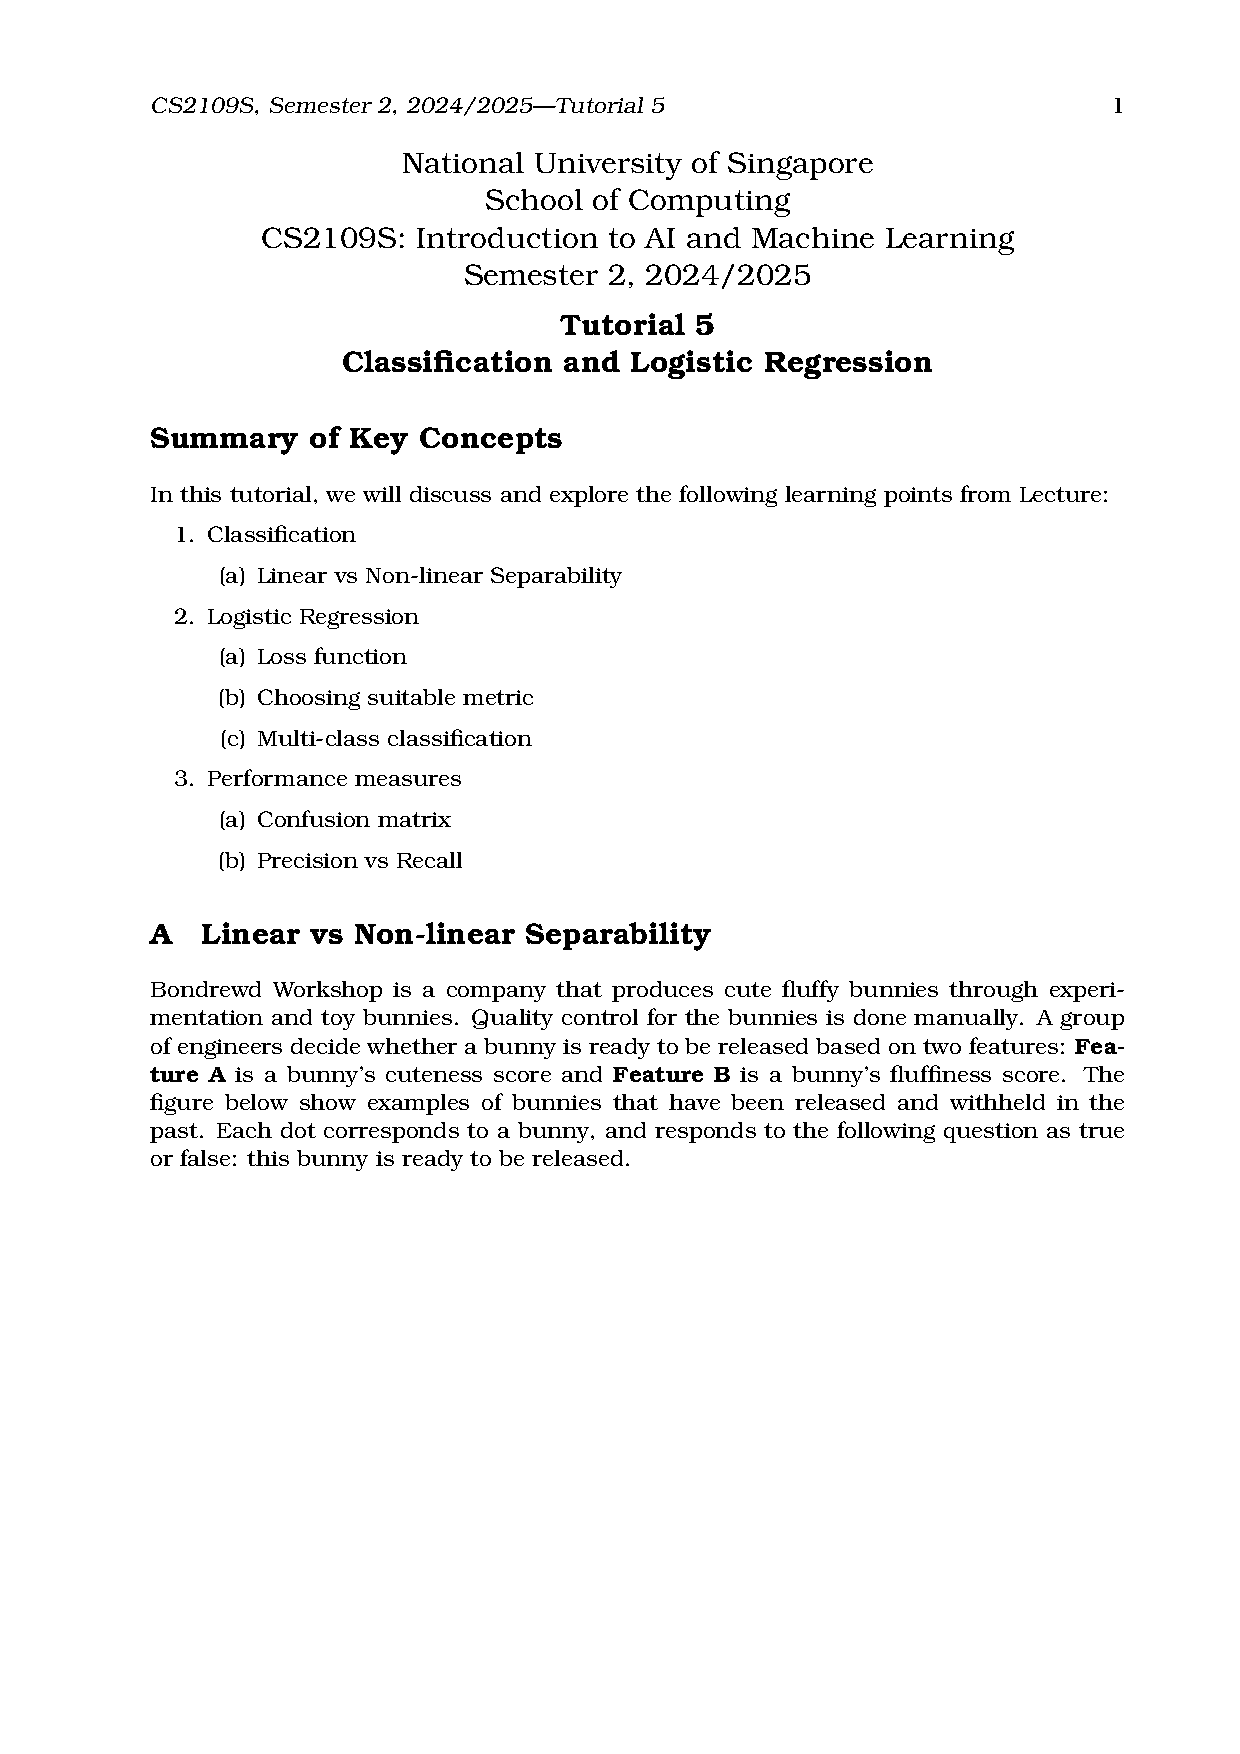
\includepdf[pages=1]{Tutorial5.pdf}
\section*{A}
\subsection*{title}
% $(|A - 2|, |B - 1|), (\frac{(A - h)^2}{a} + \frac{(B - k)^2}{b})$a
$(A, B, A^2, B^2)$ required term for the ellipse equation
\subsection*{title}
$(A, B)$
\includepdf[pages=2]{Tutorial5.pdf}
\section*{B}
\subsection*{}
\[p(h_w(x) = 1|x) = h_w(x) = \frac{1}{1 + e^{-w^Tx}}\]
\[p(h_w(x) = 0|x) = 1 - h_w(x) = 1 - \frac{1}{1 + e^{-w^Tx}} = \frac{e^{-w^Tx}}{1 + e^{-w^Tx}}\]
\subsection*{}
First expand the matrix representation:

\begin{align*}
  \ln \left( p(h_w(x) = 1 \mid x) \right) 
      &= \ln(1) - \ln \left( 1 + e^{-w^T x} \right) \\
      &= \ln(1) - \ln \left( 1 + e^{-\sum_{i = 1}^{N} w_i x_i} \right)
  \end{align*}
  
  \begin{align*}
  \frac{\partial \ln p_1}{\partial w_i} 
      &= -\frac{\partial}{\partial w_i} \ln ( 1 + e^{-\sum_{i = 1}^{N} w_i x_i} ) \\
      &= \frac{1}{\ln ( 1 + e^{-\sum_{i = 1}^{N} w_i x_i} )} 
         \frac{\partial}{\partial w_i} e^{-\sum_{i = 1}^{N} w_i x_i}\\
      &= 
  \end{align*}
\includepdf[pages=3]{Tutorial5.pdf}
\section*{C}
\subsection*{}

\includepdf[pages=4]{Tutorial5.pdf}
\includepdf[pages=5]{Tutorial5.pdf}


\end{document}
